% !TEX root = ../thesis.tex

\chapter{Evaluation}

\paragraph{Ausblick:}
Dieses Kapitel dient der Evaluation der im vorangegangenen Kapitel erläuterten Klassifikationen. Dies geschieht durch verschiedene Evaluationsmetriken, welche in diesem Kapitel vorgestellt werden. Ebenfalls umfasst dieses Kapitel einen Vergleich der Klassifikatoren zu einer nicht-featurebasierten Methode und eine Erläuterung der Herausforderungen und Limitationen, die mit der Erarbeitung der vorangegangenen Kapitel einhergingen.
\\
\hrule

\section{Herausforderungen und Limitationen}

\section{Vergleich der Klassifikatoren}

Der Vergleich der Klassifikatoren erfolgt unter Zuhilfenahme von Evaluationsmetriken, die im nachfolgenden Abschnitt vorgestellt werden. Die Diskussion der Ergebnisse der Evaluation erfolgt in Abschnitt 5.2.2.

\subsection{Evaluationsmetriken}

Die zum Vergleich der Klassifikatoren erhobenen Evaluationmetriken entstammen dem Themengebiet des Information Retrieval und gelten als Standardmesswerte für ihren Einsatzzweck \cite{Sammut2017}. Ein Großteil dieser Metriken lässt sich anhand von Werten einer sogenannten Konfusionsmatrix berechnen. Im Falle einer binären Klassifikation, wie in dieser Arbeit, besteht diese Matrix aus vier Gruppen, deren Werte angeben, ob der jeweilige Klassifikator ein Objekt korrekt oder falsch einer der beiden Zielklassen zuordnen konnte \cite{Sammut2017}. Im Zusammenhang mit solchen Matrizen werden die beiden Zielklassen \glqq positiv\grqq{} und \glqq negativ\grqq{} genannt. Für diese Arbeit werden die positive Klasse dem Label \glqq fehlerfrei\grqq und die negative Klasse dem Label \glqq defekt\grqq{} zugeordnet. Die Form einer allgemeinen Konfusionsmatrix ist in Abbildung XX dargestellt.

\begin{figure}[]
    \centering
    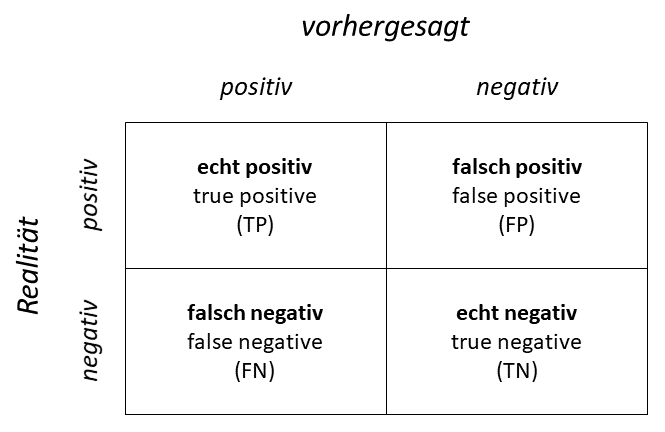
\includegraphics[width=0.7\textwidth]{images/Confusion}
    \caption{allgemeine Konfusionsmatrix\label{fig:confu}}
\end{figure}

Sowohl scitkit-learn als auch WEKA besitzen die Option, Konfisionsmatrizen zu den durchgeführten Tests der Klassifikatoren auszugeben. Anhand der Werte der Zuordnungen zu den Gruppen wurden die folgenden Evaluationsmetriken berechnet: 

\begin{itemize}
\item Treffergenauigkeit (Accuracy)
\\Dieser Wert misst die Treffergenauigkeit der Vorhersagen des Klassifikators und gibt an, inwieweit dessen Vorhersagen mit der modellierten Realität übereinstimmen \cite{Sammut2017}.
\\\[Accuracy = \frac{TP+TN}{TP+TN+FP+FN}\]
\item Echt-Positiv-Rate / Trefferquote (TP-Rate / Recall)
\\Dieser Wert gibt den Anteil der korrekt als positiv gewerteten Vorhersagen an. \cite{Alpaydin2010}
\\\[TP-Rate = \frac{TP}{TP+FN}\]
\item Falsch-Positiv-Rate (FP-Rate)
\\Dieser Wert gibt den Anteil der fälschlicherweise als positiv gewerteten Vorhersagen an. \cite{Alpaydin2010}
\\\[FP-Rate = \frac{FP}{FP+TN}\]
\item Positiver Vorhersagewert (Precision)
\\ Dieser Wert gibt die Anzahl der positiven Vorhersagen an, die auch tatsächlich zur positiven Klasse gehören \cite{Sammut2017}.
\\\[Precision = \frac{TP}{TP+FP}\]
\item F-Maß (F-Score)
\\ Dieser Wert berechnet das harmonische Mittel zwischen den Werten Precision und Recall und liegt somit zwischen diesen beiden Werten, jedoch näher am kleineren Wert \cite{Sammut2017}.
\\\[F-Score = \frac{2TP}{2TP+FP+FN}\]
\item ROC-Bereich (ROC-Area)
\\Dieser Wert unterliegt der Messung der ROC-Kurve (ROC =  Receiver operating characteristic, Betriebsverhalten des Empfängers), welche das Verhältnis zwischen der TP-Rate und der FP-Rate modelliert \cite{Sammut2017}. Die ROC-Area, auch AUC (area under curce, Bereich unter der Kurve) genannt, evaluiert den Bereich unter dieser Kurve mit einem Wert zwischen 0 (alle Negativwerte rangieren vor allen Positivwerten) und 1 (alle Positivwerte rangieren vor allen Negativwerten) \cite{Sammut2017}.
\item PRC-Bereich (PRC-Area)
\\Dieser Wert unterliegt der Messung der PRC (Precision-Recall-Curve), welche die Werte der Precision und des Recalls gegenüberstellt. Die Messung des Bereiches unter dieser Kurve erfolgt analog zur ROC-Area.
\end{itemize}

\subsection{Ergebnisse und Diskussion}

\begin{table}
\centering
\caption{Konfusionsmatrizen (scikit-learn)}
\label{tab:mat-scikit}
\resizebox{\linewidth}{!}{%
\begin{tabular}{>{\centering\hspace{0pt}}p{0.077\linewidth}>{\hspace{0pt}}p{0.233\linewidth}>{\centering\hspace{0pt}}p{0.146\linewidth}>{\centering\hspace{0pt}}p{0.102\linewidth}>{\centering\hspace{0pt}}p{0.081\linewidth}|>{\centering\hspace{0pt}}p{0.146\linewidth}>{\centering\hspace{0pt}}p{0.102\linewidth}>{\centering\arraybackslash\hspace{0pt}}p{0.096\linewidth}}
\multicolumn{1}{>{\hspace{0pt}}p{0.077\linewidth}}{}            &                       & \multicolumn{3}{>{\centering\hspace{0pt}}p{0.329\linewidth}|}{\textbf{Feat-Datenset} } & \multicolumn{3}{>{\centering\arraybackslash\hspace{0pt}}p{0.344\linewidth}}{\textbf{File-Datenset} }  \\ 
\cline{2-8}
\multicolumn{1}{>{\centering\hspace{0pt}}p{0.077\linewidth}|}{} & \textbf{Ermittelt -\textgreater}  & \textbf{Fehlerfrei}  & \textbf{Defekt}  & \textbf{Total}                               & \textbf{Fehlerfrei}  & \textbf{Defekt}  & \textbf{Total}                                              \\ 
\hline
\multirow{3}{0.077\linewidth}{\hspace{0pt}\Centering{}DT}       & Realität fehlerfrei   & 2221                 & 185              & 2406                                         & 13009                & 138              & 13147                                                       \\
                                                                & Realität defekt       & 224                  & 388              & 612                                          & 726                  & 4169             & 4895                                                        \\
                                                                & Total                 & 2445                 & 573              & 3018                                         & 13735                & 4307             & 18042                                                       \\ 
\hline
\multirow{3}{0.077\linewidth}{\hspace{0pt}\Centering{}KNN}      & Realität fehlerfrei   & 2952                 & 110              & 3062                                         & 20398                & 1592             & 21990                                                       \\
                                                                & Realität defekt       & 394                  & 317              & 711                                          & 1125                 & 6954             & 8079                                                        \\
                                                                & Total                 & 3346                 & 427              & 3773                                         & 21523                & 8546             & 30069                                                       \\ 
\hline
\multirow{3}{0.077\linewidth}{\hspace{0pt}\Centering{}NB}       & Realität fehlerfrei   & 2489                 & 533              & 3022                                         & 14618                & 7395             & 22013                                                       \\
                                                                & Realität defekt       & 695                  & 56               & 751                                          & 2426                 & 5630             & 8056                                                        \\
                                                                & Total                 & 3184                 & 589              & 3773                                         & 17044                & 13025            & 30069                                                       \\ 
\hline
\multirow{3}{0.077\linewidth}{\hspace{0pt}\Centering{}NN}       & Realität fehlerfrei   & 4689                 & 168              & 4857                                         & 16959                & 693              & 17652                                                       \\
                                                                & Realität defekt       & 480                  & 481              & 961                                          & 1752                 & 4652             & 6404                                                        \\
                                                                & Total                 & 5169                 & 649              & 5818                                         & 18711                & 5345             & 24056                                                       \\ 
\hline
\multirow{3}{0.077\linewidth}{\hspace{0pt}\Centering{}RC}       & Realität fehlerfrei   & 3036                 & 17               & 3053                                         & 13073                & 102              & 13175                                                       \\
                                                                & Realität defekt       & 637                  & 83               & 720                                          & 4705                 & 102              & 4807                                                        \\
                                                                & Total                 & 3673                 & 100              & 3772                                         & 17778                & 204              & 17982                                                       \\ 
\hline
\multirow{3}{0.077\linewidth}{\hspace{0pt}\Centering{}RF}       & Realität fehlerfrei   & 2372                 & 69               & 2441                                         & 13296                & 70               & 13366                                                       \\
                                                                & Realität defekt       & 165                  & 412              & 577                                          & 188                  & 4488             & 4676                                                        \\
                                                                & Total                 & 2357                 & 481              & 3018                                         & 13484                & 4558             & 18042                                                       \\ 
\hline
\multirow{3}{0.077\linewidth}{\hspace{0pt}\Centering{}SGD}      & Realität fehlerfrei   & 1792                 & 41               & 1833                                         & 7291                 & 10296            & 17587                                                       \\
                                                                & Realität defekt       & 356                  & 75               & 431                                          & 717                  & 5752             & 6469                                                        \\
                                                                & Total                 & 1833                 & 116              & 2264                                         & 8008                 & 16048            & 24056                                                       \\ 
\hline
\multirow{3}{0.077\linewidth}{\hspace{0pt}\Centering{}SVM}      & Realität fehlerfrei   & 2996                 & 45               & 3041                                         & 21948                & 210              & 22158                                                       \\
                                                                & Realität defekt       & 541                  & 191              & 732                                          & 7704                 & 207              & 7911                                                        \\
                                                                & Total                 & 3537                 & 236              & 3773                                         & 29652                & 417              & 30069                                                      
\end{tabular}
}
\end{table}

\begin{table}
\centering
\caption{Konfusionsmatrizen (WEKA)}
\label{tab:mat-weka}
\resizebox{\linewidth}{!}{%
\begin{tabular}{>{\centering\hspace{0pt}}p{0.075\linewidth}>{\hspace{0pt}}p{0.225\linewidth}>{\centering\hspace{0pt}}p{0.141\linewidth}>{\centering\hspace{0pt}}p{0.098\linewidth}>{\centering\hspace{0pt}}p{0.091\linewidth}|>{\centering\hspace{0pt}}p{0.143\linewidth}>{\centering\hspace{0pt}}p{0.1\linewidth}>{\centering\arraybackslash\hspace{0pt}}p{0.112\linewidth}}
\multicolumn{1}{>{\hspace{0pt}}p{0.075\linewidth}}{}            &                       & \multicolumn{3}{>{\centering\hspace{0pt}}p{0.329\linewidth}|}{\textbf{Feat-Datenset} } & \multicolumn{3}{>{\centering\arraybackslash\hspace{0pt}}p{0.355\linewidth}}{\textbf{File-Datenset} }  \\ 
\cline{2-8}
\multicolumn{1}{>{\centering\hspace{0pt}}p{0.075\linewidth}|}{} & \textbf{Ermittelt -\textgreater}  & \textbf{Fehlerfrei}  & \textbf{Defekt}  & \textbf{Total}                               & \textbf{Fehlerfrei}  & \textbf{Defekt}  & \textbf{Total}                                              \\ 
\hline
\multirow{3}{0.075\linewidth}{\hspace{0pt}\Centering{}J48}      & Realität fehlerfrei   & 11569                & 580              & 12149                                        & 86805                & 1231             & 88036                                                       \\
                                                                & Realität defekt       & 1094                 & 1848             & 2942                                         & 1745                 & 30495            & 32240                                                       \\
                                                                & Total                 & 12663                & 2428             & 15091                                        & 88550                & 31726            & 120276                                                      \\ 
\hline
\multirow{3}{0.075\linewidth}{\hspace{0pt}\Centering{}KNN}      & Realität fehlerfrei   & 11284                & 865              & 12149                                        & 84426                & 3610             & 88036                                                       \\
                                                                & Realität defekt       & 1024                 & 1917             & 2941                                         & 5163                 & 27077            & 32240                                                       \\
                                                                & Total                 & 12308                & 2782             & 15087                                        & 89589                & 30687            & 120276                                                      \\ 
\hline
\multirow{3}{0.075\linewidth}{\hspace{0pt}\Centering{}LR}       & Realität fehlerfrei   & 3554                 & 103              & 3657                                         & 13081                & 157              & 13238                                                       \\
                                                                & Realität defekt       & 571                  & 299              & 870                                          & 4625                 & 178              & 4803                                                        \\
                                                                & Total                 & 4125                 & 402              & 4527                                         & 17706                & 335              & 18041                                                       \\ 
\hline
\multirow{3}{0.075\linewidth}{\hspace{0pt}\Centering{}NB}       & Realität fehlerfrei   & 11806                & 343              & 12149                                        & 25807                & 534              & 26341                                                       \\
                                                                & Realität defekt       & 1978                 & 963              & 2941                                         & 8993                 & 749              & 9742                                                        \\
                                                                & Total                 & 13784                & 1306             & 15090                                        & 34800                & 1283             & 36083                                                       \\ 
\hline
\multirow{3}{0.075\linewidth}{\hspace{0pt}\Centering{}NN}       & Realität fehlerfrei   & 1671                 & 120              & 1791                                         & 21981                & 0                & 21981                                                       \\
                                                                & Realität defekt       & 194                  & 278              & 472                                          & 8088                 & 0                & 8088                                                        \\
                                                                & Total                 & 1865                 & 398              & 2263                                         & 30069                & 0                & 30069                                                       \\ 
\hline
\multirow{3}{0.075\linewidth}{\hspace{0pt}\Centering{}RF}       & Realität fehlerfrei   & 11741                & 408              & 12149                                        & 13161                & 77               & 13238                                                       \\
                                                                & Realität defekt       & 865                  & 2076             & 2941                                         & 174                  & 4629             & 4803                                                        \\
                                                                & Total                 & 12606                & 2484             & 15090                                        & 13335                & 4706             & 19841                                                       \\ 
\hline
\multirow{3}{0.075\linewidth}{\hspace{0pt}\Centering{}SGD}      & Realität fehlerfrei   & 3623                 & 34               & 3657                                         & 13237                & 1                & 13238                                                       \\
                                                                & Realität defekt       & 686                  & 184              & 870                                          & 4803                 & 0                & 4803                                                        \\
                                                                & Total                 & 4319                 & 218              & 4537                                         & 18040                & 1                & 18041                                                       \\ 
\hline
\multirow{3}{0.075\linewidth}{\hspace{0pt}\Centering{}SVM}      & Realität fehlerfrei   & 3652                 & 5                & 3657                                         & 13238                & 0                & 13238                                                       \\
                                                                & Realität defekt       & 801                  & 69               & 870                                          & 4803                 & 0                & 4803                                                        \\
                                                                & Total                 & 4453                 & 74               & 7427                                         & 18041                & 0                & 18041                                                      
\end{tabular}
}
\end{table}

\begin{figure}
  \centering
  \subfloat[][DT (scikit)]{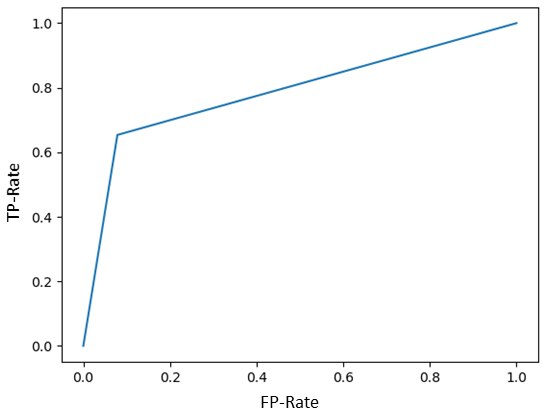
\includegraphics[width=0.25\linewidth]{images/dt_scikit}}
  \subfloat[][J48 (WEKA)]{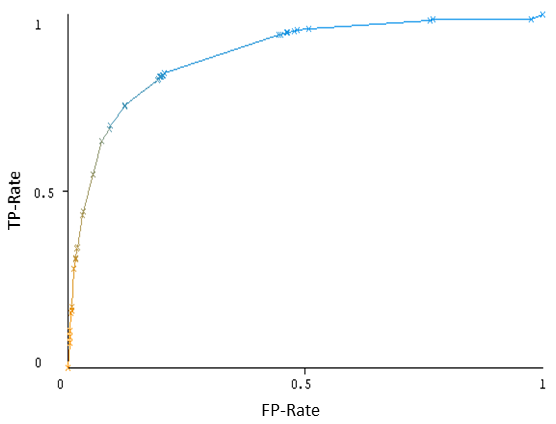
\includegraphics[width=0.25\linewidth]{images/j48_weka}}
  \subfloat[][NN (scikit)]{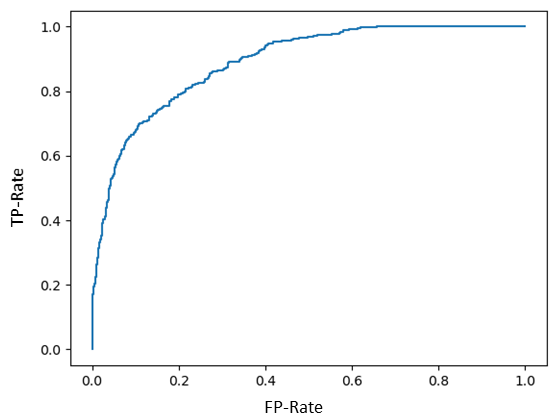
\includegraphics[width=0.25\linewidth]{images/nn_scikit}}
  \subfloat[][NN (WEKA)]{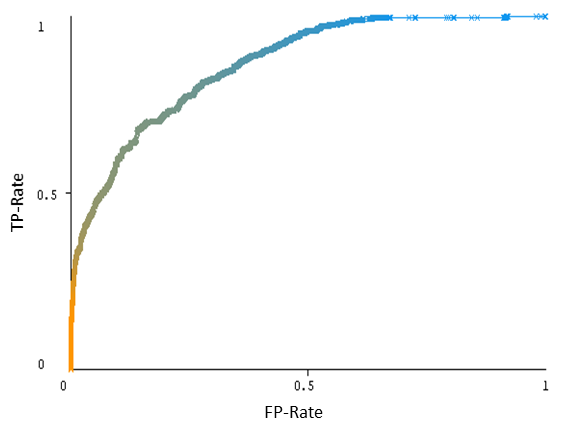
\includegraphics[width=0.25\linewidth]{images/nn_weka}}
  \qquad
  \subfloat[][KNN (scikit)]{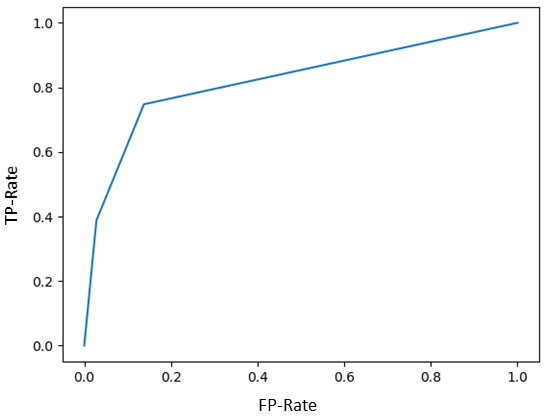
\includegraphics[width=0.25\linewidth]{images/knn_scikit}}
  \subfloat[][KNN (WEKA)]{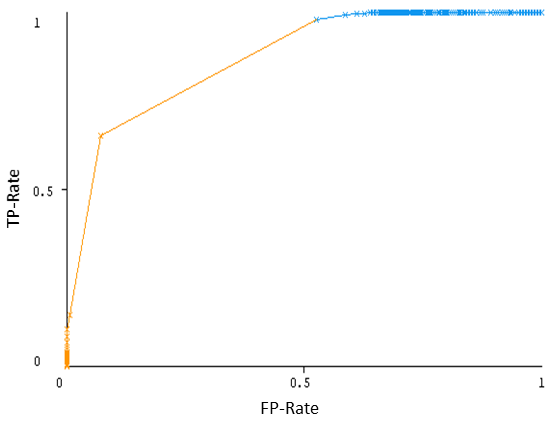
\includegraphics[width=0.25\linewidth]{images/knn_weka}}
  \subfloat[][RF (scikit)]{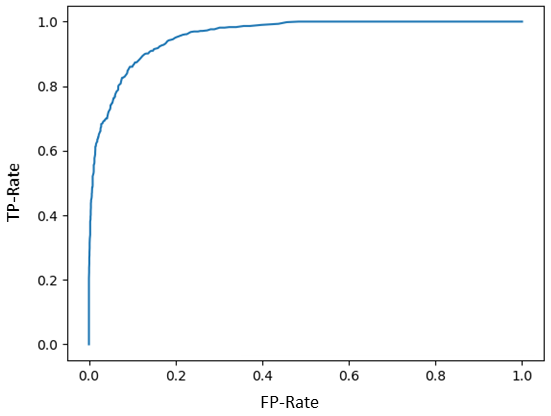
\includegraphics[width=0.25\linewidth]{images/rf_scikit}}
  \subfloat[][RF (WEKA)]{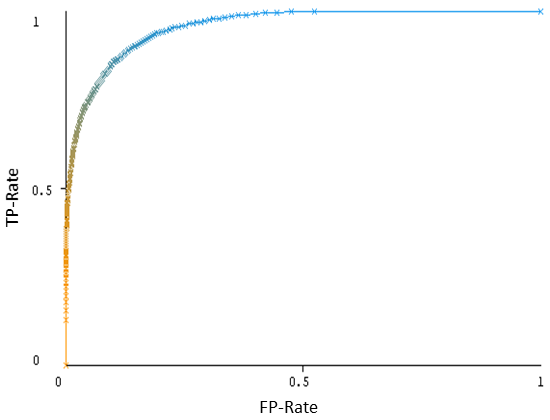
\includegraphics[width=0.25\linewidth]{images/rf_weka}}
  \qquad
  \subfloat[][RC (scikit)]{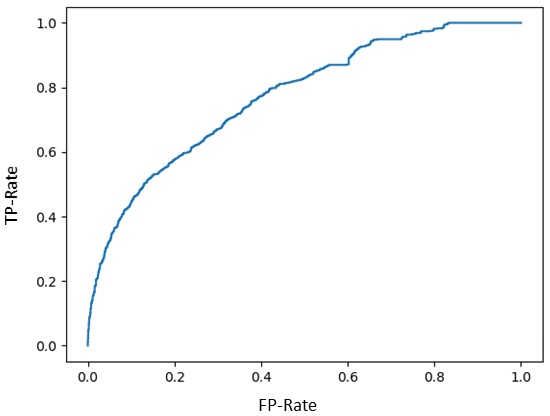
\includegraphics[width=0.25\linewidth]{images/rc_scikit}}
  \subfloat[][LR (WEKA)]{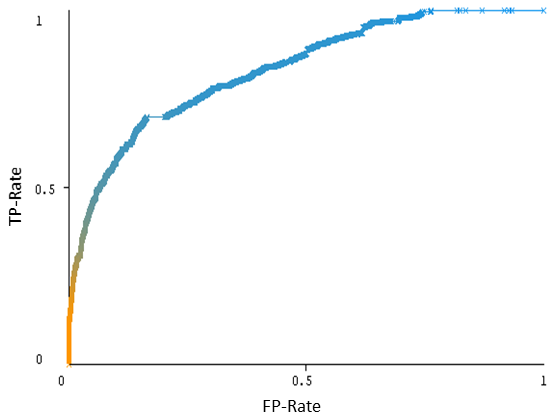
\includegraphics[width=0.25\linewidth]{images/lr_weka}}
  \subfloat[][SGD (scikit)]{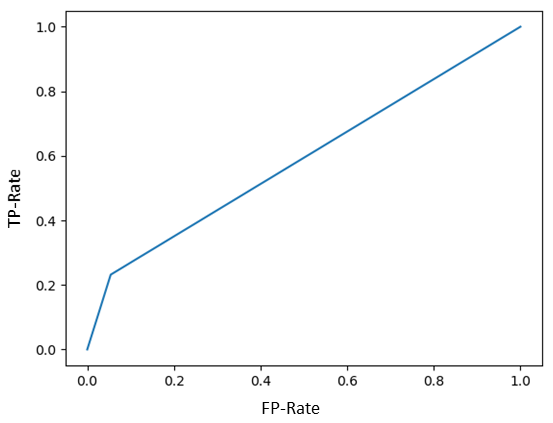
\includegraphics[width=0.25\linewidth]{images/sgd_scikit}}
  \subfloat[][SGD (WEKA)]{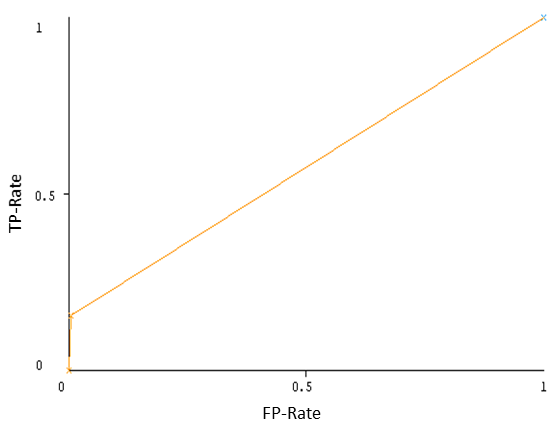
\includegraphics[width=0.25\linewidth]{images/sgd_weka}}
  \qquad
  \subfloat[][NB (scikit)]{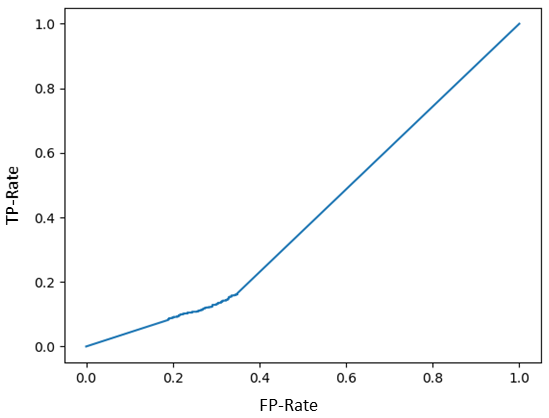
\includegraphics[width=0.25\linewidth]{images/nb_scikit}}
  \subfloat[][NB (WEKA)]{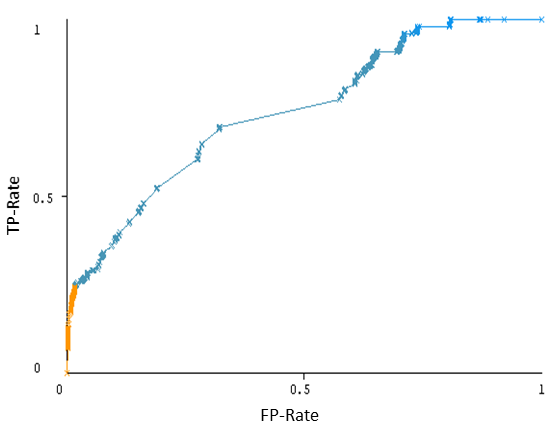
\includegraphics[width=0.25\linewidth]{images/nb_weka}}
  \subfloat[][SVM (scikit)]{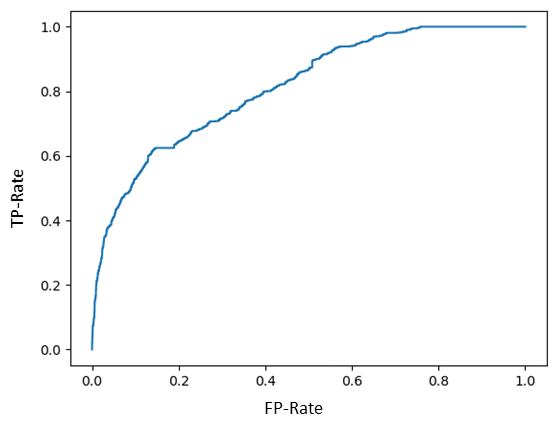
\includegraphics[width=0.25\linewidth]{images/svm_scikit}}
  \subfloat[][SVM (WEKA)]{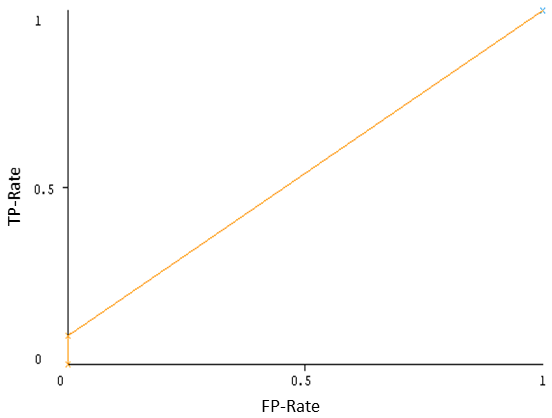
\includegraphics[width=0.25\linewidth]{images/svm_weka}}
  \caption{ROC-Kurven der Klassifikatoren des featurebasierten Datensets}
\end{figure}

\begin{figure}
  \centering
  \subfloat[][DT (scikit)]{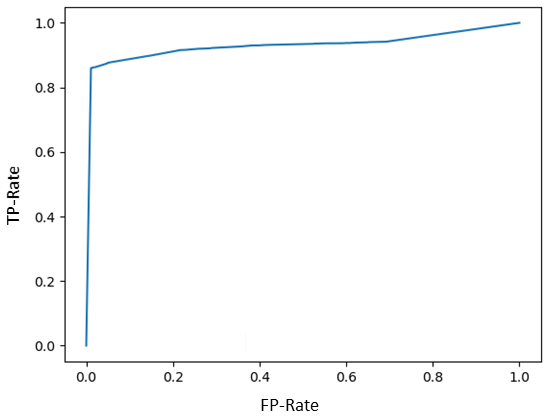
\includegraphics[width=0.25\linewidth]{images/dt_scikit_file}}
  \subfloat[][J48 (WEKA)]{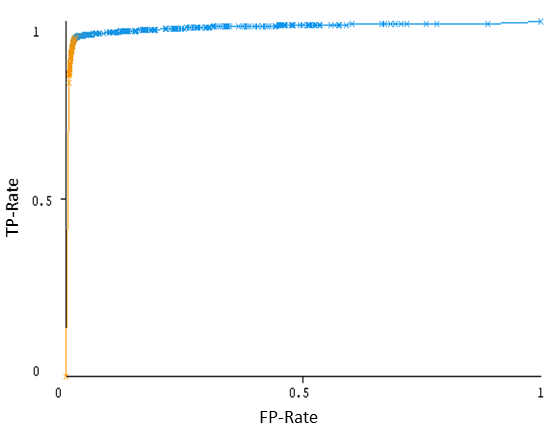
\includegraphics[width=0.25\linewidth]{images/j48_weka_file}}
  \subfloat[][NN (scikit)]{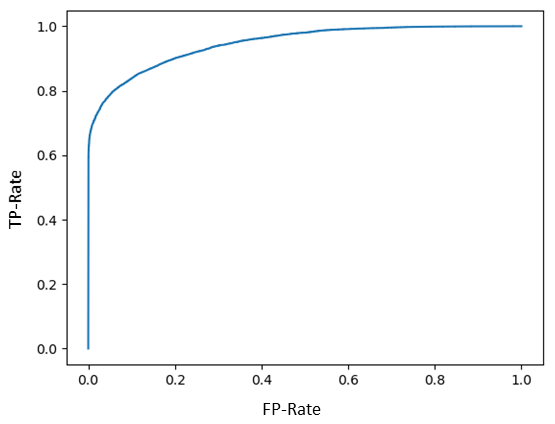
\includegraphics[width=0.25\linewidth]{images/nn_scikit_file}}
  \subfloat[][NN (WEKA)]{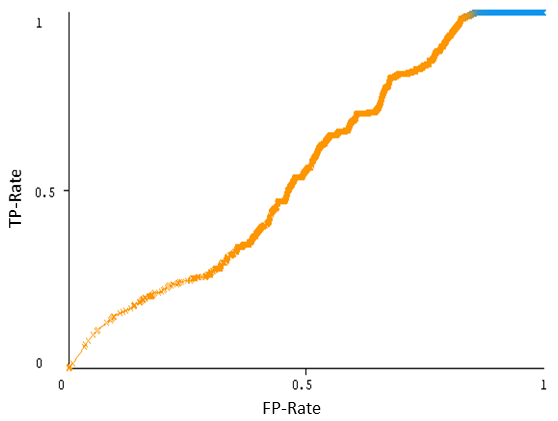
\includegraphics[width=0.25\linewidth]{images/nn_weka_file}}
  \qquad
  \subfloat[][KNN (scikit)]{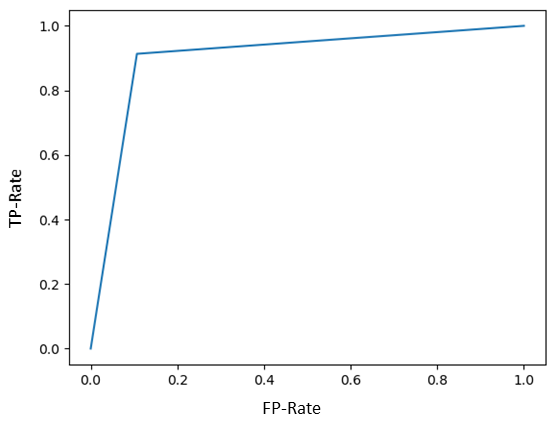
\includegraphics[width=0.25\linewidth]{images/knn_scikit_file}}
  \subfloat[][KNN (WEKA)]{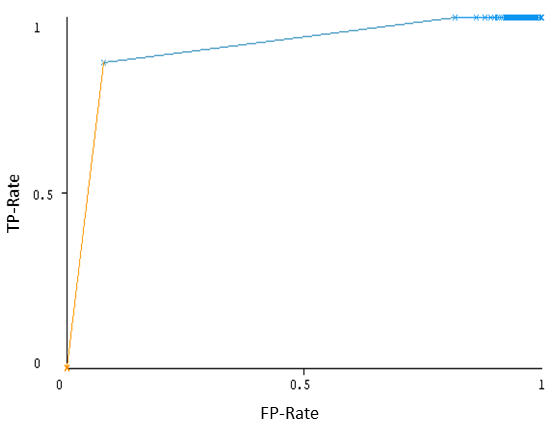
\includegraphics[width=0.25\linewidth]{images/knn_weka_file}}
  \subfloat[][RF (scikit)]{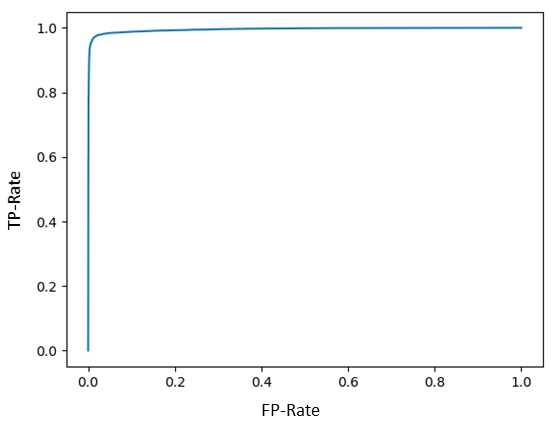
\includegraphics[width=0.25\linewidth]{images/rf_scikit_file}}
  \subfloat[][RF (WEKA)]{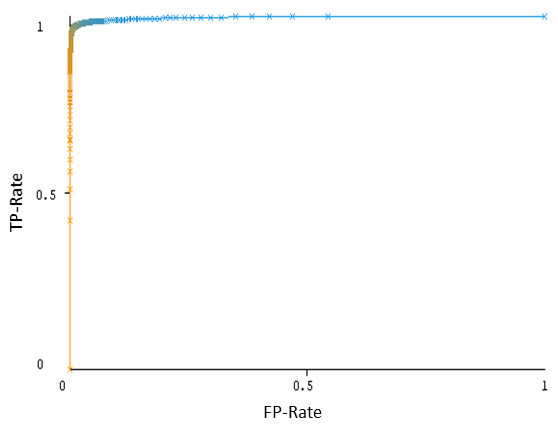
\includegraphics[width=0.25\linewidth]{images/rf_weka_file}}
  \qquad
  \subfloat[][RC (scikit)]{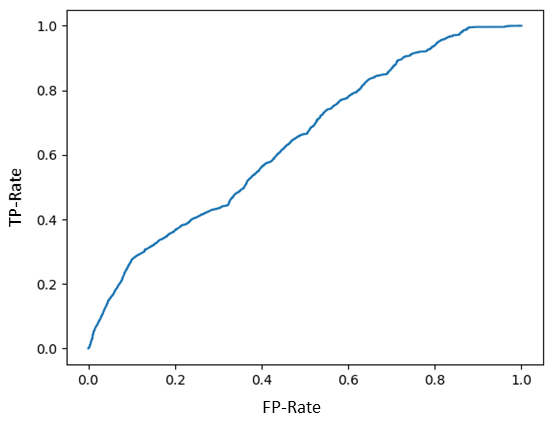
\includegraphics[width=0.25\linewidth]{images/rc_scikit_file}}
  \subfloat[][LR (WEKA)]{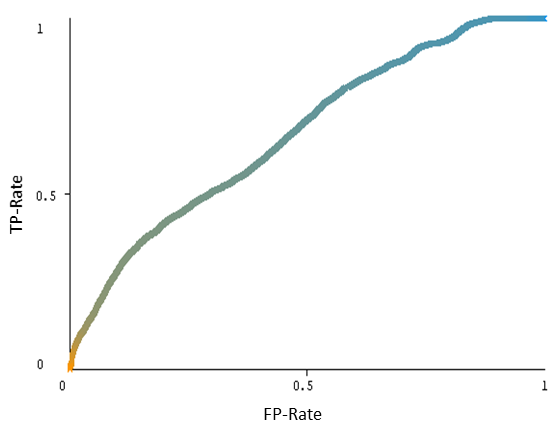
\includegraphics[width=0.25\linewidth]{images/lr_weka_file}}
  \subfloat[][SGD (scikit)]{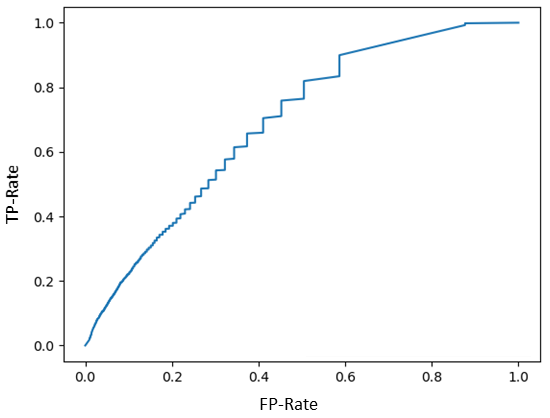
\includegraphics[width=0.25\linewidth]{images/sgd_scikit_file}}
  \subfloat[][SGD (WEKA)]{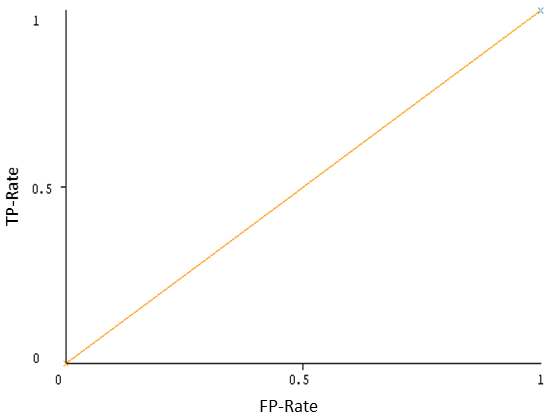
\includegraphics[width=0.25\linewidth]{images/sgd_weka_file}}
  \qquad
  \subfloat[][NB (scikit)]{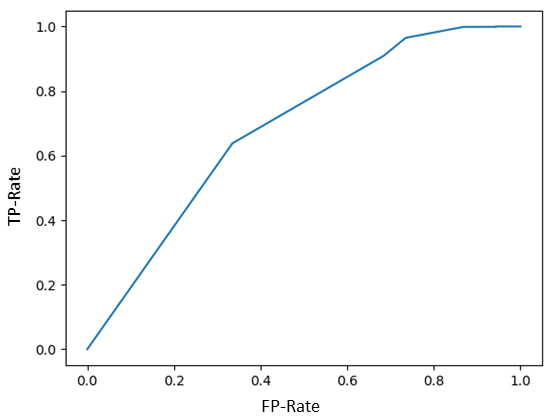
\includegraphics[width=0.25\linewidth]{images/nb_scikit_file}}
  \subfloat[][NB (WEKA)]{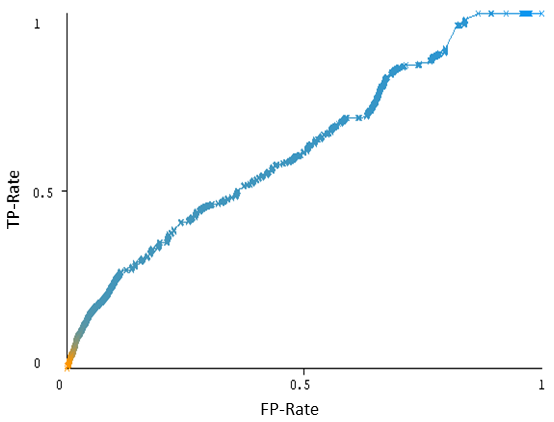
\includegraphics[width=0.25\linewidth]{images/nb_weka_file}}
  \subfloat[][SVM (scikit)]{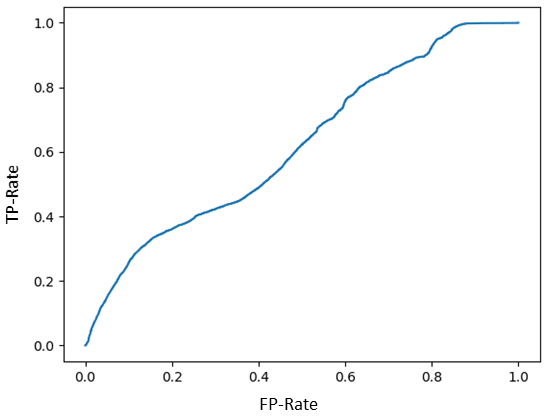
\includegraphics[width=0.25\linewidth]{images/svm_scikit_file}}
  \subfloat[][SVM (WEKA)]{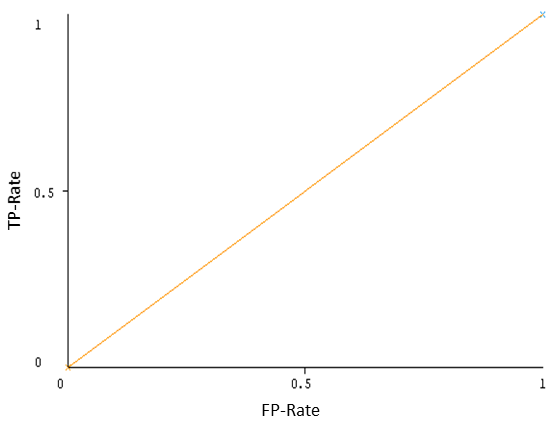
\includegraphics[width=0.25\linewidth]{images/svm_weka_file}}
  \caption{ROC-Kurven der Klassifikatoren des dateibasierten Datensets}
\end{figure}

\begin{figure}[]
    \centering
    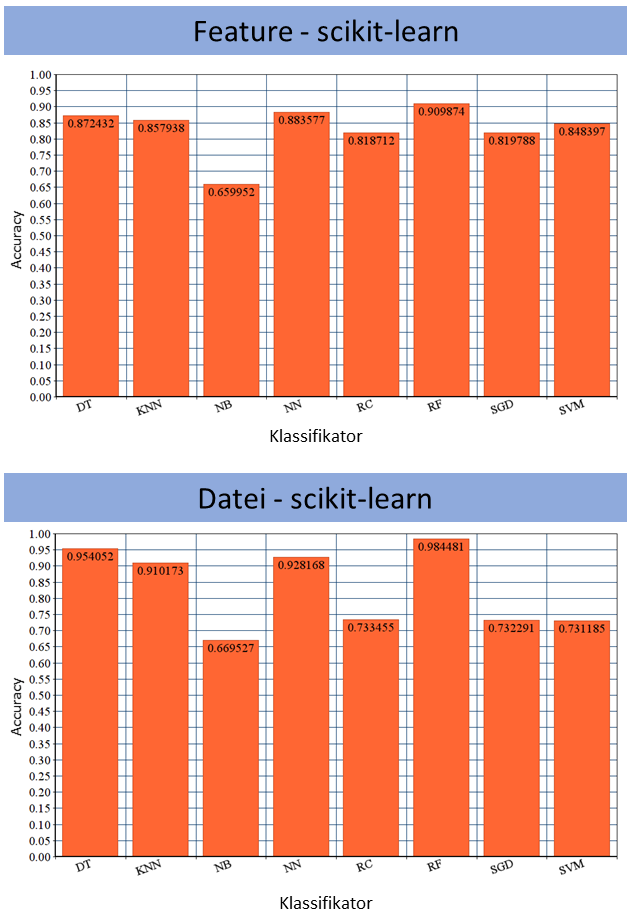
\includegraphics[width=0.8\textwidth]{images/Final_scikit}
    \caption{Vergleich der Accuracies zwischen den Datensets der scikit-Klassifikatoren\label{fig:final-scikit}}
\end{figure}

\begin{figure}[]
    \centering
    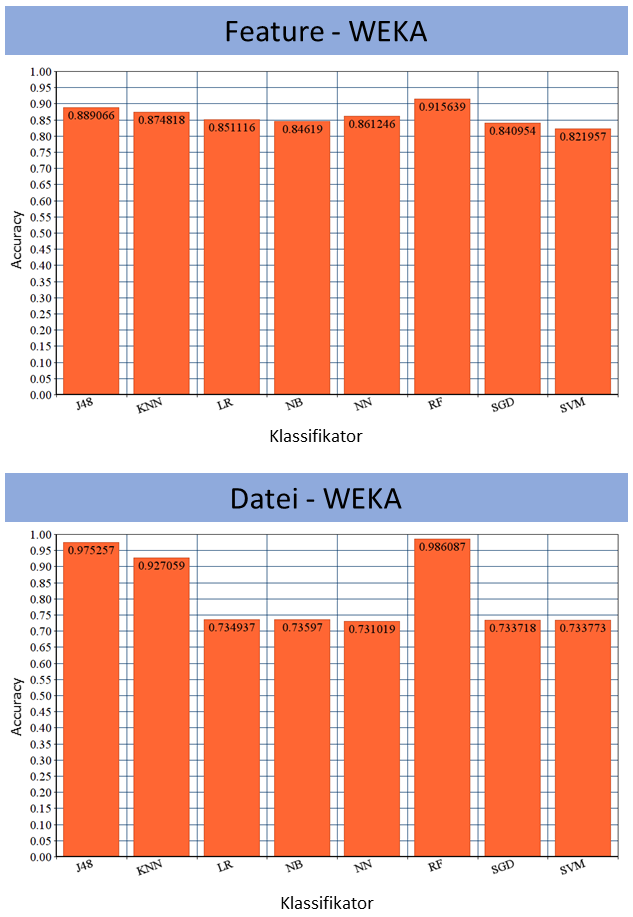
\includegraphics[width=0.8\textwidth]{images/Final_weka}
    \caption{Vergleich der Accuracies zwischen den Werkzeugen der WEKA-Klassifikatoren\label{fig:final-weka}}
\end{figure}

\begin{table}
\centering
\caption{Ergebnisse der Evaluationsmetriken auf Basis der Konfusionsmatrix (scikit-learn)}
\label{tab:met-scikit}
\resizebox{\linewidth}{!}{%
\begin{tabular}{>{\centering\hspace{0pt}}p{0.083\linewidth}>{\hspace{0pt}}p{0.164\linewidth}>{\centering\hspace{0pt}}p{0.158\linewidth}>{\centering\hspace{0pt}}p{0.112\linewidth}>{\centering\hspace{0pt}}p{0.098\linewidth}|>{\centering\hspace{0pt}}p{0.158\linewidth}>{\centering\hspace{0pt}}p{0.112\linewidth}>{\centering\arraybackslash\hspace{0pt}}p{0.1\linewidth}}
\multicolumn{1}{>{\hspace{0pt}}p{0.083\linewidth}}{}       &                                                       & \multicolumn{3}{>{\centering\hspace{0pt}}p{0.368\linewidth}|}{\textbf{Feat-Datenset} } & \multicolumn{3}{>{\centering\arraybackslash\hspace{0pt}}p{0.37\linewidth}}{\textbf{File-Datenset} }  \\ 
\cline{3-8}
                                                           & \multicolumn{1}{>{\hspace{0pt}}p{0.164\linewidth}|}{} & \textbf{Fehlerfrei}  & \textbf{Defekt}  & \textbf{gew.}\par{}\textbf{Mittel}           & \textbf{Fehlerfrei}  & \textbf{Defekt}  & \textbf{gew.}\par{}\textbf{Mittel}                         \\ 
\hline
\multirow{7}{0.083\linewidth}{\hspace{0pt}\Centering{}DT}  & TP-Rate                                               & 0,92                 & 0,63             & 0,86                                         & 0,99                 & 0,85             & 0,95                                                       \\
                                                           & FP-Rate                                               & 0,37                 & 0,08             & 0,31                                         & 0,15                 & 0,01             & 0,11                                                       \\
                                                           & Precision                                             & 0,91                 & 0,68             & 0,86                                         & 0,95                 & 0,97             & 0,95                                                       \\
                                                           & Recall                                                & 0,92                 & 0,63             & 0,86                                         & 0,99                 & 0,85             & 0,95                                                       \\
                                                           & F-Score                                               & 0,92                 & 0,65             & 0,86                                         & 0,97                 & 0,91             & 0,95                                                       \\
                                                           & ROC-Area                                              & 0,78                 & 0,78             & 0,78                                         & 0,92                 & 0,92             & 0,92                                                       \\
                                                           & PRC-Area                                              & 0,76                 & 0,50             & 0,71                                         & 0,72                 & 0,86             & 0,76                                                       \\ 
\hline
\multirow{7}{0.083\linewidth}{\hspace{0pt}\Centering{}KNN} & TP-Rate                                               & 0,96                 & 0,45             & 0,87                                         & 0,93                 & 0,86             & 0,91                                                       \\
                                                           & FP-Rate                                               & 0,55                 & 0,04             & 0,46                                         & 0,14                 & 0,07             & 0,12                                                       \\
                                                           & Precision                                             & 0,88                 & 0,74             & 0,86                                         & 0,95                 & 0,81             & 0,91                                                       \\
                                                           & Recall                                                & 0,96                 & 0,45             & 0,87                                         & 0,93                 & 0,86             & 0,91                                                       \\
                                                           & F-Score                                               & 0,92                 & 0,56             & 0,85                                         & 0,94                 & 0,84             & 0,91                                                       \\
                                                           & ROC-Area                                              & 0,82                 & 0,82             & 0,82                                         & 0,89                 & 0,89             & 0,89                                                       \\
                                                           & PRC-Area                                              & 0,79                 & 0,44             & 0,72                                         & 0,69                 & 0,74             & 0,71                                                       \\ 
\hline
\multirow{7}{0.083\linewidth}{\hspace{0pt}\Centering{}NB}  & TP-Rate                                               & 0,82                 & 0,07             & 0,67                                         & 0,66                 & 0,70             & 0,67                                                       \\
                                                           & FP-Rate                                               & 0,93                 & 0,18             & 0,78                                         & 0,30                 & 0,34             & 0,31                                                       \\
                                                           & Precision                                             & 0,78                 & 0,10             & 0,65                                         & 0,86                 & 0,43             & 0,74                                                       \\
                                                           & Recall                                                & 0,82                 & 0,07             & 0,67                                         & 0,66                 & 0,70             & 0,67                                                       \\
                                                           & F-Score                                               & 0,80                 & 0,08             & 0,66                                         & 0,75                 & 0,53             & 0,69                                                       \\
                                                           & ROC-Area                                              & 0,40                 & 0,40             & 0,40                                         & 0,72                 & 0,72             & 0,72                                                       \\
                                                           & PRC-Area                                              & 0,82                 & 0,19             & 0,69                                         & 0,68                 & 0,38             & 0,59                                                       \\ 
\hline
\multirow{7}{0.083\linewidth}{\hspace{0pt}\Centering{}NN}  & TP-Rate                                               & 0,97                 & 0,50             & 0,89\textasciitilde{}                        & 0,96                 & 0,73             & 0,90                                                       \\
                                                           & FP-Rate                                               & 0,50                 & 0,03             & 0,42                                         & 0,27                 & 0,04             & 0,21                                                       \\
                                                           & Precision                                             & 0,91                 & 0,74             & 0,88                                         & 0,91                 & 0,87             & 0,90                                                       \\
                                                           & Recall                                                & 0,97                 & 0,50             & 0,89                                         & 0,96                 & 0,73             & 0,90                                                       \\
                                                           & F-Score                                               & 0,94                 & 0,60             & 0,88                                         & 0,93                 & 0,79             & 0,90                                                       \\
                                                           & ROC-Area                                              & 0,90                 & 0,90             & 0,90                                         & 0,95                 & 0,95             & 0,95                                                       \\
                                                           & PRC-Area                                              & 0,81                 & 0,45             & 0,76                                         & 0,71                 & 0,71             & 0,71                                                       \\ 
\hline
\multirow{7}{0.083\linewidth}{\hspace{0pt}\Centering{}RC}  & TP-Rate                                               & 0,99                 & 0,16             & 0,83                                         & 0,99                 & 0,02             & 0,73                                                       \\
                                                           & FP-Rate                                               & 0,88                 & 0,01             & 0,72                                         & 0,98                 & 0,01             & 0,72                                                       \\
                                                           & Precision                                             & 0,83                 & 0,83             & 0,83                                         & 0,73                 & 0,50             & 0,67                                                       \\
                                                           & Recall                                                & 0,99                 & 0,12             & 0,83                                         & 0,99                 & 0,02             & 0,73                                                       \\
                                                           & F-Score                                               & 0,90                 & 0,20             & 0,77                                         & 0,84                 & 0,04             & 0,63                                                       \\
                                                           & ROC-Area                                              & 0,55                 & 0,55             & 0,55                                         & 0,51                 & 0,51             & 0,51                                                       \\
                                                           & PRC-Area                                              & 0,81                 & 0,26             & 0,70                                         & 0,73                 & 0,27             & 0,61                                                       \\ 
\hline
\multirow{7}{0.083\linewidth}{\hspace{0pt}\Centering{}RF}  & TP-Rate                                               & 0,97                 & 0,71             & 0,82                                         & 0,99                 & 0,96             & 0,99                                                       \\
                                                           & FP-Rate                                               & 0,29                 & 0,03             & 0,24                                         & 0,04                 & 0,01             & 0,03                                                       \\
                                                           & Precision                                             & 0,93                 & 0,86             & 0,92                                         & 0,99                 & 0,98             & 0,99                                                       \\
                                                           & Recall                                                & 0,97                 & 0,71             & 0,92                                         & 0,99                 & 0,96             & 0,99                                                       \\
                                                           & F-Score                                               & 0,95                 & 0,78             & 0,92                                         & 0,99                 & 0,97             & 0,99                                                       \\
                                                           & ROC-Area                                              & 0,96                 & 0,96             & 0,96                                         & 0,98                 & 0,98             & 0,98                                                       \\
                                                           & PRC-Area                                              & 0,79                 & 0,67             & 0,77                                         & 0,74                 & 0,96             & 0,79                                                       \\ 
\hline
\multirow{7}{0.083\linewidth}{\hspace{0pt}\Centering{}SGD} & TP-Rate                                               & 0,98                 & 0,17             & 0,82                                         & 0,41                 & 0,89             & 0,54                                                       \\
                                                           & FP-Rate                                               & 0,83                 & 0,02             & 0,67                                         & 0,11                 & 0,59             & 0,54                                                       \\
                                                           & Precision                                             & 0,83                 & 0,65             & 0,80                                         & 0,91                 & 0,36             & 0,76                                                       \\
                                                           & Recall                                                & 0,98                 & 0,17             & 0,82                                         & 0,41                 & 0,89             & 0,54                                                       \\
                                                           & F-Score                                               & 0,90                 & 0,27             & 0,78                                         & 0,57                 & 0,51             & 0,55                                                       \\
                                                           & ROC-Area                                              & 0,58                 & 0,58             & 0,58                                         & 0,68                 & 0,68             & 0,68                                                       \\
                                                           & PRC-Area                                              & 0,80                 & 0,27             & 0,70                                         & 0,68                 & 0,35             & 0,59                                                       \\ 
\hline
\multirow{7}{0.083\linewidth}{\hspace{0pt}\Centering{}SVM} & TP-Rate                                               & 0,99                 & 0,26             & 0,84                                         & 0,99                 & 0,03             & 0,74                                                       \\
                                                           & FP-Rate                                               & 0,74                 & 0,01             & 0,84                                         & 0,97                 & 0,01             & 0,72                                                       \\
                                                           & Precision                                             & 0,85                 & 0,81             & 0,84                                         & 0,74                 & 0,50             & 0,68                                                       \\
                                                           & Recall                                                & 0,99                 & 0,26             & 0,84                                         & 0,99                 & 0,03             & 0,74                                                       \\
                                                           & F-Score                                               & 0,91                 & 0,39             & 0,81                                         & 0,85                 & 0,05             & 0,64                                                       \\
                                                           & ROC-Area                                              & 0,62                 & 0,62             & 0,62                                         & 0,51                 & 0,51             & 0,51                                                       \\
                                                           & PRC-Area                                              & 0,80                 & 0,35             & 0,71                                         & 0,73                 & 0,27             & 0,61                                                      
\end{tabular}
}
\end{table}

\begin{table}
\centering
\caption{Ergebnisse der Evaluationsmetriken auf Basis der Konfusionsmatrix (WEKA)}
\label{tab:met-weka}
\resizebox{\linewidth}{!}{%
\begin{tabular}{>{\centering\hspace{0pt}}p{0.085\linewidth}>{\hspace{0pt}}p{0.168\linewidth}>{\centering\hspace{0pt}}p{0.152\linewidth}>{\centering\hspace{0pt}}p{0.112\linewidth}>{\centering\hspace{0pt}}p{0.1\linewidth}|>{\centering\hspace{0pt}}p{0.154\linewidth}>{\centering\hspace{0pt}}p{0.112\linewidth}>{\centering\arraybackslash\hspace{0pt}}p{0.102\linewidth}}
\multicolumn{1}{>{\hspace{0pt}}p{0.085\linewidth}}{\textbf{} } & \textbf{}                                             & \multicolumn{3}{>{\centering\hspace{0pt}}p{0.364\linewidth}|}{\textbf{Feat-Datenset} } & \multicolumn{3}{>{\centering\arraybackslash\hspace{0pt}}p{0.368\linewidth}|}{\textbf{File-Datenset} }  \\ 
\cline{3-8}
                                                               & \multicolumn{1}{>{\hspace{0pt}}p{0.168\linewidth}|}{} & \textbf{fehlerfrei} & \textbf{defekt} & \textbf{gew.}\par{}\textbf{Mittel}             & \textbf{fehlerfrei} & \textbf{defekt} & \textbf{gew.}\par{}\textbf{Mittel}                             \\ 
\hline
\multirow{7}{0.085\linewidth}{\hspace{0pt}\Centering{}DT}      & TP-Rate                                               & 0,92                & 0,63            & 0,89                                           & 0,99                & 0,95            & 0,98                                                           \\
                                                               & FP-Rate                                               & 0,37                & 0,05            & 0,31                                           & 0,05                & 0,01            & 0,04                                                           \\
                                                               & Precision                                             & 0,91                & 0,76            & 0,88                                           & 0,98                & 0,96            & 0,98                                                           \\
                                                               & Recall                                                & 0,95                & 0,62            & 0,89                                           & 0,99                & 0,95            & 0,98                                                           \\
                                                               & F-Score                                               & 0,93                & 0,69            & 0,89                                           & 0,98                & 0,95            & 0,98                                                           \\
                                                               & ROC-Area                                              & 0,89                & 0,89            & 0,89                                           & 0,98                & 0,98            & 0,98                                                           \\
                                                               & PRC-Area                                              & 0,96                & 0,71            & 0,91                                           & 0,98                & 0,62            & 0,98                                                           \\ 
\hline
\multirow{7}{0.085\linewidth}{\hspace{0pt}\Centering{}KNN}     & TP-Rate                                               & 0,93                & 0,65            & 0,88                                           & 0,96                & 0,84            & 0,93                                                           \\
                                                               & FP-Rate                                               & 0,35                & 0,07            & 0,29                                           & 0,16                & 0,04            & 0,13                                                           \\
                                                               & Precision                                             & 0,92                & 0,69            & 0,72                                           & 0,94                & 0,88            & 0,93                                                           \\
                                                               & Recall                                                & 0,93                & 0,65            & 0,88                                           & 0,96                & 0,84            & 0,93                                                           \\
                                                               & F-Score                                               & 0,92                & 0,67            & 0,87                                           & 0,95                & 0,86            & 0,93                                                           \\
                                                               & ROC-Area                                              & 0,87                & 0,87            & 0,87                                           & 0,91                & 0,91            & 0,91                                                           \\
                                                               & PRC-Area                                              & 0,95                & 0,59            & 0,88                                           & 0,95                & 0,80            & 0,91                                                           \\ 
\hline
\multirow{7}{0.085\linewidth}{\hspace{0pt}\Centering{}LR}      & TP-Rate                                               & 0,97                & 0,34            & 0,85                                           & 0,99                & 0,04            & 0,74                                                           \\
                                                               & FP-Rate                                               & 0,66                & 0,03            & 0,54                                           & 0,96                & 0,01            & 0,71                                                           \\
                                                               & Precision                                             & 0,86                & 0,74            & 0,84                                           & 0,74                & 0,53            & 0,68                                                           \\
                                                               & Recall                                                & 0,92                & 0,34            & 0,85                                           & 0,99                & 0,04            & 0,74                                                           \\
                                                               & F-Score                                               & 0,91                & 0,47            & 0,83                                           & 0,85                & 0,07            & 0,64                                                           \\
                                                               & ROC-Area                                              & 0,83                & 0,83            & 0,83                                           & 0,62                & 0,62            & 0,62                                                           \\
                                                               & PRC-Area                                              & 0,95                & 0,63            & 0,89                                           & 0,83                & 0,38            & 0,71                                                           \\ 
\hline
\multirow{7}{0.085\linewidth}{\hspace{0pt}\Centering{}NB}      & TP-Rate                                               & 0,92                & 0,33            & 0,85                                           & 0,98                & 0,08            & 0,74                                                           \\
                                                               & FP-Rate                                               & 0,67                & 0,03            & 0,55                                           & 0,92                & 0,02            & 0,68                                                           \\
                                                               & Precision                                             & 0,86                & 0,74            & 0,83                                           & 0,74                & 0,58            & 0,70                                                           \\
                                                               & Recall                                                & 0,97                & 0,33            & 0,85                                           & 0,98                & 0,08            & 0,74                                                           \\
                                                               & F-Score                                               & 0,91                & 0,45            & 0,82                                           & 0,88                & 0,14            & 0,65                                                           \\
                                                               & ROC-Area                                              & 0,73                & 0,73            & 0,73                                           & 0,62                & 0,62            & 0,62                                                           \\
                                                               & PRC-Area                                              & 0,91                & 0,51            & 0,83                                           & 0,82                & 0,38            & 0,70                                                           \\ 
\hline
\multirow{7}{0.085\linewidth}{\hspace{0pt}\Centering{}NN}      & TP-Rate                                               & 0,93                & 0,59            & 0,86                                           & 1,00                & 0,00            & 0,73                                                           \\
                                                               & FP-Rate                                               & 0,41                & 0,07            & 0,34                                           & 1,00                & 0,00            & 0,73                                                           \\
                                                               & Precision                                             & 0,90                & 0,70            & 0,86                                           & 0,73                & ?               & ?                                                              \\
                                                               & Recall                                                & 0,93                & 0,59            & 0,86                                           & 1,00                & 0,00            & 0,73                                                           \\
                                                               & F-Score                                               & 0,91                & 0,64            & 0,86                                           & 0,85                & ?               & ?                                                              \\
                                                               & ROC-Area                                              & 0,82                & 0,82            & 0,82                                           & 0,55                & 0,55            & 0,55                                                           \\
                                                               & PRC-Area                                              & 0,96                & 0,72            & 0,91                                           & 0,80                & 0,30            & 0,67                                                           \\ 
\hline
\multirow{7}{0.085\linewidth}{\hspace{0pt}\Centering{}RF}      & TP-Rate                                               & 0,97                & 0,71            & 0,92                                           & 0,99                & 0,96            & 0,99                                                           \\
                                                               & FP-Rate                                               & 0,29                & 0,03            & 0,24                                           & 0,04                & 0,01            & 0,03                                                           \\
                                                               & Precision                                             & 0,93                & 0,84            & 0,91                                           & 0,99                & 0,98            & 0,99                                                           \\
                                                               & Recall                                                & 0,97                & 0,71            & 0,92                                           & 0,99                & 0,96            & 0,99                                                           \\
                                                               & F-Score                                               & 0,95                & 0,77            & 0,91                                           & 0,99                & 0,97            & 0,99                                                           \\
                                                               & ROC-Area                                              & 0,96                & 0,96            & 0,96                                           & 0,99                & 0,99            & 0,99                                                           \\
                                                               & PRC-Area                                              & 0,99                & 0,87            & 0,97                                           & 1,00                & 0,99            & 1,00                                                           \\ 
\hline
\multirow{7}{0.085\linewidth}{\hspace{0pt}\Centering{}SGD}     & TP-Rate                                               & 0,99                & 0,21            & 0,84                                           & 1,00                & 0,00            & 0,73                                                           \\
                                                               & FP-Rate                                               & 0,79                & 0,01            & 0,64                                           & 1,00                & 0,00            & 0,73                                                           \\
                                                               & Precision                                             & 0,84                & 0,84            & 0,84                                           & 0,73                & 0,00            & 0,538                                                          \\
                                                               & Recall                                                & 0,99                & 0,41            & 0,84                                           & 1,00                & 0,00            & 0,734                                                          \\
                                                               & F-Score                                               & 0,91                & 0,34            & 0,80                                           & 0,85                & 0,00            & 0,621                                                          \\
                                                               & ROC-Area                                              & 0,60                & 0,60            & 0,60                                           & 0,50                & 0,50            & 0,50                                                           \\
                                                               & PRC-Area                                              & 0,84                & 0,33            & 0,74                                           & 0,73                & 0,27            & 0,61                                                           \\ 
\hline
\multirow{7}{0.085\linewidth}{\hspace{0pt}\Centering{}SVM}     & TP-Rate                                               & 1,00                & 0,08            & 0,82                                           & 1,00                & 0,00            & 0,73                                                           \\
                                                               & FP-Rate                                               & 0,92                & 0,00            & 0,74                                           & 1,00                & 0,00            & 0,73                                                           \\
                                                               & Precision                                             & 0,82                & 0,93            & 0,84                                           & 0,73                & ?               & ?                                                              \\
                                                               & Recall                                                & 1,00                & 0,08            & 0,82                                           & 1,00                & 0,00            & 0,73                                                           \\
                                                               & F-Score                                               & 0,90                & 0,15            & 0,76                                           & 0,85                & ?               & ?                                                              \\
                                                               & ROC-Area                                              & 0,54                & 0,54            & 0,54                                           & 0,50                & 0,50            & 0,50                                                           \\
                                                               & PRC-Area                                              & 0,82                & 0,25            & 0,71                                           & 0,73                & 0,27            & 0,61                                                          
\end{tabular}
}
\end{table}


\section{Vergleich zu nicht-featurebasierten Methoden}

\begin{table}[]
\centering
\caption{Übersicht der berechneten Metriken nach \cite{Moser2008}}
\label{tab:eval-metrics}
\resizebox{\textwidth}{!}{%
\begin{tabular}{lll}
\hline
\multicolumn{1}{|l}{\textbf{Name}} & \textbf{Abkürzung} & \multicolumn{1}{l|}{\textbf{Beschreibung}}                                                                                                                                                                       \\ \hline
REVISIONS                          & revi               & Anzahl der Revisionen (Bearbeitungen) der Datei.                                                                                                                                                                 \\
REFACTORINGS                       & refa               & \begin{tabular}[c]{@{}l@{}}Anzahl der Fälle, in denen die Datei in einem Refactoring\\ involviert war.  Basierend auf Analyse der Commit-Nachricht\\ auf das Vorhandensein des Begriffs "refactor".\end{tabular} \\
BUGFIXES                           & bugf               & \begin{tabular}[c]{@{}l@{}}Anzahl der Fälle, in denen die Datei in einer Fehlerbehebung\\ involviert war.\end{tabular}                                                                                           \\
AUTHORS                            & auth               & \begin{tabular}[c]{@{}l@{}}Anzahl der verschiedenen Autoren, die die Datei in das\\ Repository eingecheckt haben.\end{tabular}                                                                                   \\
LOC\_ADDED                         & addl               & \begin{tabular}[c]{@{}l@{}}Summe der zur Datei hinzugefügten Codezeilen über\\ alle Revisionen.\end{tabular}                                                                                                     \\
MAX\_LOC\_ADDED                    & addm               & \begin{tabular}[c]{@{}l@{}}Maximale Anzahl von Codezeilen, die für alle Revisionen\\ hinzugefügt wurden.\end{tabular}                                                                                            \\
AVE\_LOC\_ADDED                    & adda               & Durchschnittlich hinzugefügte Codezeilen pro Revision.                                                                                                                                                           \\
LOC\_DELETED                       & reml               & \begin{tabular}[c]{@{}l@{}}Summe der von der Datei entfernten Codezeilen über alle\\ Revisionen.\end{tabular}                                                                                                    \\
MAX\_LOC\_DELETED                  & remm               & \begin{tabular}[c]{@{}l@{}}Maximale Anzahl von Codezeilen, die für alle Revisionen\\ entfernt wurden.\end{tabular}                                                                                               \\
AVE\_LOC\_DELETED                  & rema               & Durchschnittlich entfernte Codezeilen pro Revision.                                                                                                                                                              \\
CODECHURN                          & cchl               & \begin{tabular}[c]{@{}l@{}}Summe von (hinzugefügte Codezeilen - entfernte Codezeilen)\\ über alle Revisionen.\end{tabular}                                                                                       \\
MAX\_CODECHURN                     & cchl               & Maximaler CODECHURN für alle Revisionen.                                                                                                                                                                         \\
AVE\_CODECHURN                     & ccha               & Durchschnittlicher CODECHURN pro Revision.                                                                                                                                                                       \\
MAX\_CHANGESET                     & maxc               & \begin{tabular}[c]{@{}l@{}}Maximale Anzahl von Dateien, die gemeinsam committed\\ wurden.\end{tabular}                                                                                                           \\
AVE\_CHANGESET                     & avgc               & \begin{tabular}[c]{@{}l@{}}Durchschnittliche Anzahl von Dateien, die gemeinsam\\ committed wurden.\end{tabular}                                                                                                  \\
AGE                                & aage               & \begin{tabular}[c]{@{}l@{}}Alter der Datei in Wochen (rückwärts zählend bis zu\\ einem bestimmten Release).\end{tabular}                                                                                         \\
WEIGHTED\_AGE                      & wage               & $Weighted Age = \frac{\sum_{i=1}^N Age(i)*LOC\_ADDED(i)}{\sum_{i=1}^N LOC\_ADDED(i)}$                                                                                                                                                                                                          
\end{tabular}%
}
\end{table}

\begin{table}
\centering
\caption{Konfusionsmatrizen der Evaluation der Klassifikatoren des klassischen Datensets}
\label{tab:class-mat}
\resizebox{\linewidth}{!}{%
\begin{tabular}{>{\centering\hspace{0pt}}p{0.114\linewidth}>{\hspace{0pt}}p{0.345\linewidth}>{\centering\hspace{0pt}}p{0.216\linewidth}>{\centering\hspace{0pt}}p{0.15\linewidth}>{\centering\arraybackslash\hspace{0pt}}p{0.166\linewidth}|} 
\cline{2-5}
\multicolumn{1}{>{\centering\hspace{0pt}}p{0.114\linewidth}|}{} & \textbf{Ermittelt -\textgreater}  & \textbf{Fehlerfrei}  & \textbf{Defekt}  & \textbf{Total}   \\ 
\hline
\multirow{3}{0.114\linewidth}{\hspace{0pt}\Centering{}J48}      & Realität fehlerfrei   & 86965                & 1071             & 88036            \\
                                                                & Realität defekt       & 1691                 & 30549            & 32240            \\
                                                                & Total                 & 88656                & 31620            & 120276           \\ 
\hline
\multirow{3}{0.114\linewidth}{\hspace{0pt}\Centering{}KNN}      & Realität fehlerfrei   & 86121                & 1915             & 88036            \\
                                                                & Realität defekt       & 3867                 & 28373            & 32240            \\
                                                                & Total                 & 89988                & 30288            & 120276           \\ 
\hline
\multirow{3}{0.114\linewidth}{\hspace{0pt}\Centering{}LR}       & Realität fehlerfrei   & 13094                & 134              & 13228            \\
                                                                & Realität defekt       & 4676                 & 137              & 4813             \\
                                                                & Total                 & 17770                & 271              & 18041            \\ 
\hline
\multirow{3}{0.114\linewidth}{\hspace{0pt}\Centering{}NB}       & Realität fehlerfrei   & 7232                 & 19102            & 26334            \\
                                                                & Realität defekt       & 527                  & 9222             & 9749             \\
                                                                & Total                 & 7759                 & 28324            & 36083            \\ 
\hline
\multirow{3}{0.114\linewidth}{\hspace{0pt}\Centering{}NN}       & Realität fehlerfrei   & 30607                & 153              & 30760            \\
                                                                & Realität defekt       & 7646                 & 3691             & 11337            \\
                                                                & Total                 & 38253                & 3844             & 42097            \\ 
\hline
\multirow{3}{0.114\linewidth}{\hspace{0pt}\Centering{}RF}       & Realität fehlerfrei   & 87694                & 342              & 88036            \\
                                                                & Realität defekt       & 936                  & 31277            & 32213            \\
                                                                & Total                 & 88630                & 31619            & 120249           \\ 
\hline
\multirow{3}{0.114\linewidth}{\hspace{0pt}\Centering{}SGD}      & Realität fehlerfrei   & 13221                & 7                & 13228            \\
                                                                & Realität defekt       & 4813                 & 0                & 4813             \\
                                                                & Total                 & 18034                & 7                & 18041            \\ 
\hline
\multirow{3}{0.114\linewidth}{\hspace{0pt}\Centering{}SVM}      & Realität fehlerfrei   & 13228                & 0                & 13228            \\
                                                                & Realität defekt       & 4813                 & 0                & 4813             \\
                                                                & Total                 & 18041                & 0                & 18041           
\end{tabular}
}
\end{table}


\begin{figure}[]
    \centering
    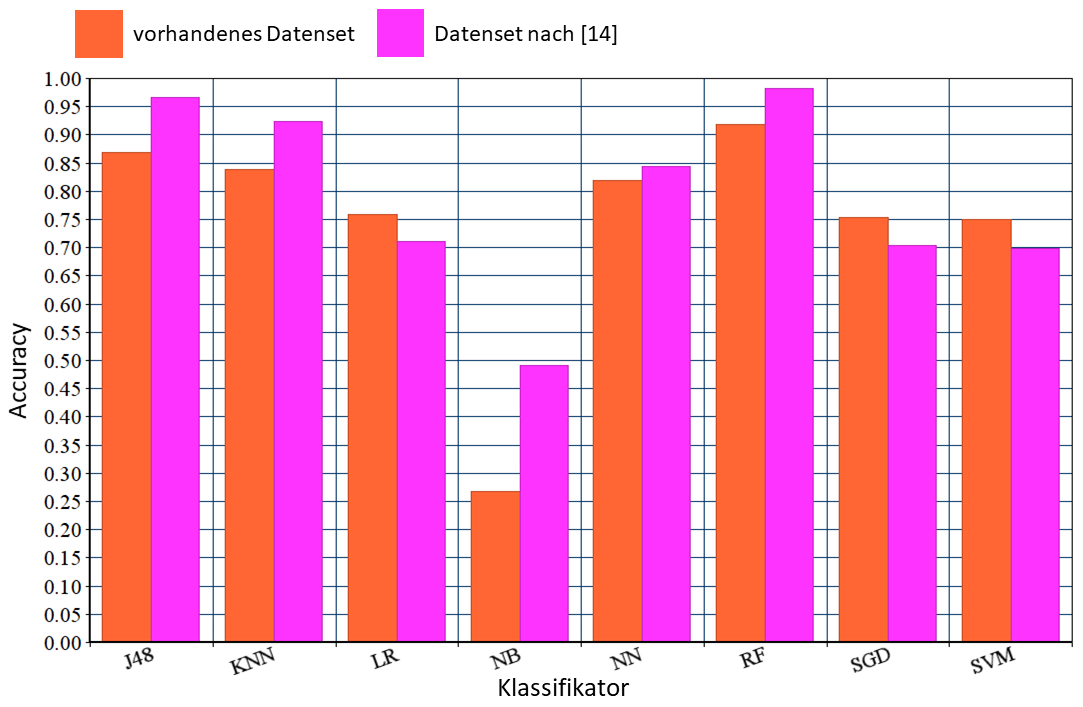
\includegraphics[width=\textwidth]{images/Klasseval}
    \caption{Übersicht der Accuracies der jeweilgen Klassifikatoren\label{fig:class-acc}}
\end{figure}

\begin{figure}
  \centering
  \subfloat[][J48]{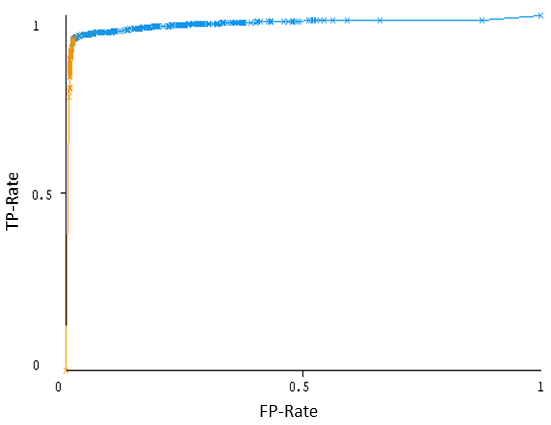
\includegraphics[width=0.25\linewidth]{images/j48_eval}}
  \subfloat[][KNN]{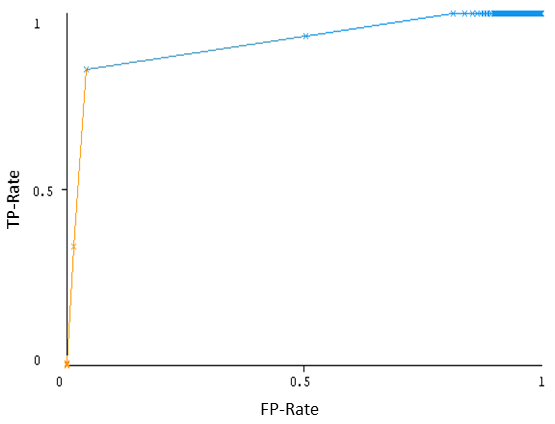
\includegraphics[width=0.25\linewidth]{images/knn_eval}}
  \subfloat[][NN]{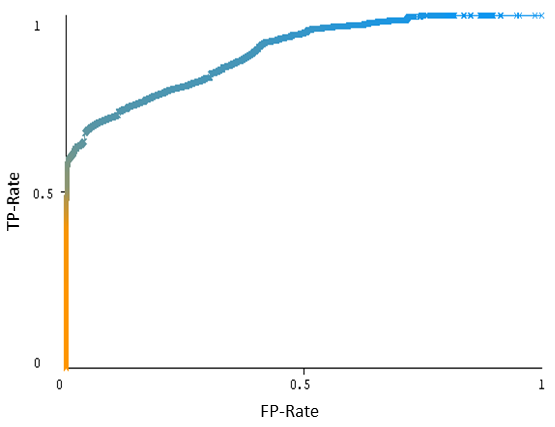
\includegraphics[width=0.25\linewidth]{images/nn_eval}}
  \subfloat[][RF]{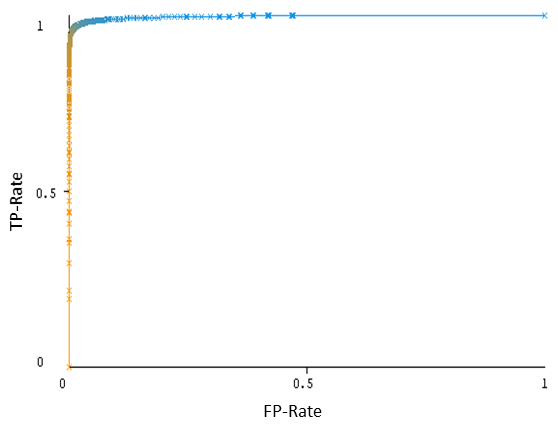
\includegraphics[width=0.25\linewidth]{images/rf_eval}}
  \qquad
  \subfloat[][LR]{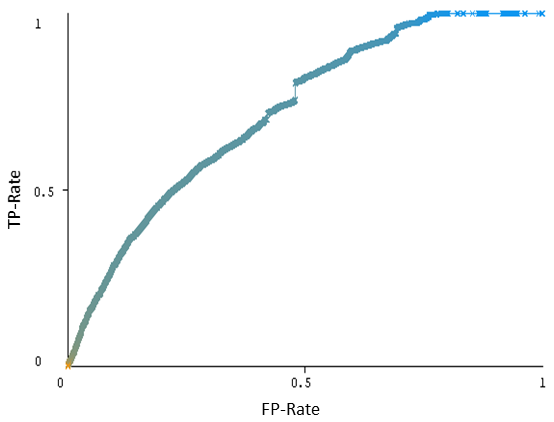
\includegraphics[width=0.25\linewidth]{images/lr_eval}}
  \subfloat[][NB]{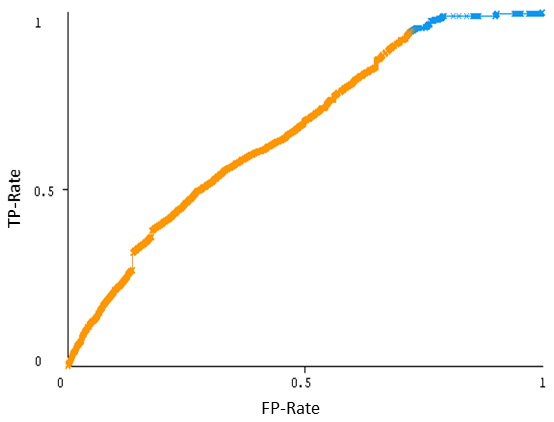
\includegraphics[width=0.25\linewidth]{images/nb_eval}}
  \subfloat[][SGD]{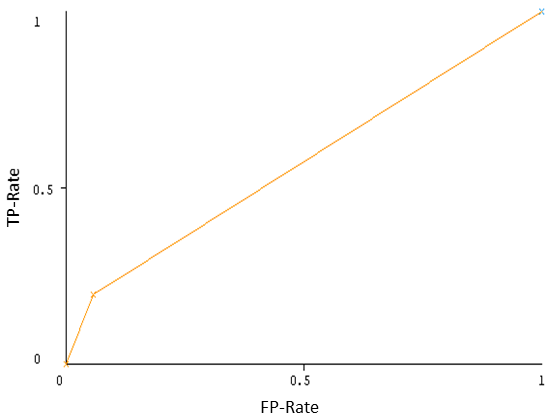
\includegraphics[width=0.25\linewidth]{images/sgd_eval}}
  \subfloat[][SVM]{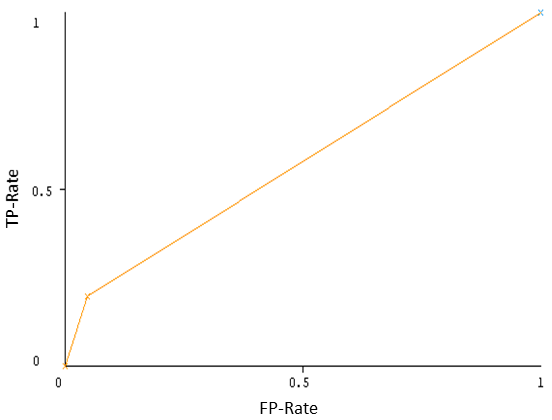
\includegraphics[width=0.25\linewidth]{images/svm_eval}}
  \caption{ROC-Kurven der Klassifikatoren}
\end{figure}


\begin{table}
\centering
\caption{Ergebnisse der Evaluationsmetriken auf Basis der Konfusionsmatrix (WEKA)}
\label{tab:class-val}
\resizebox{\linewidth}{!}{%
\begin{tabular}{>{\centering\hspace{0pt}}p{0.137\linewidth}>{\hspace{0pt}}p{0.268\linewidth}>{\centering\hspace{0pt}}p{0.245\linewidth}>{\centering\hspace{0pt}}p{0.179\linewidth}>{\centering\arraybackslash\hspace{0pt}}p{0.162\linewidth}|} 
\cline{3-5}
 & \multicolumn{1}{>{\hspace{0pt}}p{0.268\linewidth}|}{} & \textbf{fehlerfrei}  & \textbf{defekt}  & \textbf{gew.}\par{}\textbf{Mittel}  \\ 
\hline
\multirow{7}{0.137\linewidth}{\hspace{0pt}\Centering{}DT} & TP-Rate & 0,99 & 0,95 & 0,98 \\
 & FP-Rate & 0,05 & 0,01 & 0,04 \\
 & Precision & 0,98 & 0,97 & 0,98 \\
 & Recall & 0,99 & 0,95 & 0,98 \\
 & F-Score & 0,98 & 0,96 & 0,98 \\
 & ROC-Area & 0,98 & 0,98 & 0,98 \\
 & PRC-Area & 0,99 & 0,96 & 0,98 \\ 
\hline
\multirow{7}{0.137\linewidth}{\hspace{0pt}\Centering{}KNN} & TP-Rate & 0,98 & 0,88 & 0,95 \\
 & FP-Rate & 0,12 & 0,02 & 0,10 \\
 & Precision & 0,96 & 0,94 & 0,95 \\
 & Recall & 0,98 & 0,88 & 0,95 \\
 & F-Score & 0,97 & 0,91 & 0,95 \\
 & ROC-Area & 0,95 & 0,95 & 0,95 \\
 & PRC-Area & 0,97 & 0,88 & 0,95 \\ 
\hline
\multirow{7}{0.137\linewidth}{\hspace{0pt}\Centering{}LR} & TP-Rate & 0,99 & 0,03 & 0,73 \\
 & FP-Rate & 0,92 & 0,01 & 0,72 \\
 & Precision & 0,74 & 0,51 & 0,68 \\
 & Recall & 0,99 & 0,03 & 0,73 \\
 & F-Score & 0,85 & 0,05 & 0,63 \\
 & ROC-Area & 0,72 & 0,72 & 0,72 \\
 & PRC-Area & 0,88 & 0,44 & 0,77 \\ 
\hline
\multirow{7}{0.137\linewidth}{\hspace{0pt}\Centering{}NB} & TP-Rate & 0,28 & 0,95 & 0,46 \\
 & FP-Rate & 0,05 & 0,73 & 0,24 \\
 & Precision & 0,93 & 0,33 & 0,77 \\
 & Recall & 0,28 & 0,95 & 0,46 \\
 & F-Score & 0,42 & 0,48 & 0,44 \\
 & ROC-Area & 0,66 & 0,66 & 0,66 \\
 & PRC-Area & 0,85 & 0,40 & 0,73 \\ 
\hline
\multirow{7}{0.137\linewidth}{\hspace{0pt}\Centering{}NN} & TP-Rate & 1,00 & 0,33 & 0,82 \\
 & FP-Rate & 0,67 & 0,01 & 0,49 \\
 & Precision & 0,80 & 0,96 & 0,84 \\
 & Recall & 1,00 & 0,33 & 0,82 \\
 & F-Score & 0,89 & 0,49 & 0,78 \\
 & ROC-Area & 0,76 & 0,76 & 0,76 \\
 & PRC-Area & 0,88 & 0,66 & 0,82 \\ 
\hline
\multirow{7}{0.137\linewidth}{\hspace{0pt}\Centering{}RF} & TP-Rate & 1,00 & 0,97 & 0,99 \\
 & FP-Rate & 0,03 & 0,00 & 0,02 \\
 & Precision & 0,99 & 0,99 & 0,99 \\
 & Recall & 1,00 & 0,97 & 0,99 \\
 & F-Score & 0,99 & 0,98 & 0,99 \\
 & ROC-Area & 1,00 & 1,00 & 1,00 \\
 & PRC-Area & 1,00 & 0,99 & 1,00 \\ 
\hline
\multirow{7}{0.137\linewidth}{\hspace{0pt}\Centering{}SGD} & TP-Rate & 1,00 & 0,00 & 0,73 \\
 & FP-Rate & 1,00 & 0,00 & 0,73 \\
 & Precision & 0,73 & 0,00 & 0,54 \\
 & Recall & 1,00 & 0,00 & 0,73 \\
 & F-Score & 0,85 & 0,00 & 0,62 \\
 & ROC-Area & 0,50 & 0,50 & 0,50 \\
 & PRC-Area & 0,73 & 0,27 & 0,61 \\ 
\hline
\multirow{7}{0.137\linewidth}{\hspace{0pt}\Centering{}SVM} & TP-Rate & 1,00 & 0,00 & 0,73 \\
 & FP-Rate & 1,00 & 0,00 & 0,73 \\
 & Precision & 0,73 & ? & ? \\
 & Recall & 1,00 & 0,00 & 0,73 \\
 & F-Score & 0,85 & ? & ? \\
 & ROC-Area & 0,50 & 0,50 & 0,50 \\
 & PRC-Area & 0,73 & 0,27 & 0,61
\end{tabular}
}
\end{table}

\cleardoublepage
